\section{Experiments}
\label{sec:experiments}

\setlength{\textfloatsep}{2pt plus 1pt minus 1pt}
\setlength{\floatsep}{2pt plus 1pt minus 1pt}
\setlength{\intextsep}{2pt plus 1pt minus 1pt}
\setlength{\dbltextfloatsep}{2pt plus 1pt minus 1pt}
\setlength{\dblfloatsep}{2pt plus 1pt minus 1pt}

We first describe our experimental setups as follows:

\textbf{Models and Benchmarks.}
Our \textsc{OpenSearch-VL} is built on three Qwen3-VL variants~\citep{Qwen3-VL}: \textit{Qwen3-VL-8B-Instruct}, \textit{Qwen3-VL-30B-A3B-Instruct}, and \textit{Qwen3-VL-32B-Instruct}. For evaluation, we use seven knowledge-intensive benchmarks from our main results:  SimpleVQA~\citep{cheng2025simplevqa}, VDR~\citep{vdr}, MMSearch~\citep{mmsearch}, LiveVQA~\citep{fu2025livevqa}, BrowseComp-VL~\citep{webwatcher}, FVQA~\citep{wang2017fvqa}, and InfoSeek~\citep{chen2023can}. Together, they cover visual entity recognition, web evidence retrieval, multi-hop reasoning, and long-tail QA.

\textbf{Baselines and Evaluation Metrics.}
We evaluate \textsc{OpenSearch-VL} against baseline types: Direct Reasoning, where the model answers from its parametric knowledge and visual perception alone; RAG Workflow, where external retrieval results are provided in-context but the reasoning remains single-pass; and Agentic Workflow, where the model autonomously interleaves reasoning with tool calls in a multimodal environment. We report Pass@1 on all seven benchmarks. Correctness is adjudicated by a \textit{GPT-4o} judge that compares the model's final response with the reference answer. To ensure fair comparison across heterogeneous answer styles, we adopt the same evaluation protocol as VDR-Bench~\citep{vdr}; the full judge prompt is provided in Figure~\ref{apdxfig:bench-judge}.

\textbf{Datasets.}
Our SFT data consists of the \textbf{36K} multi-turn trajectories synthesized by the procedure in Sec.~\ref{sec:trajectory-synthesis}. For RL training, we randomly sample \textbf{8K} examples from the VQA pool after the staged filtering and enhancement process in Sec.~\ref{sec:filtering-enhancement}, ensuring that these examples are disjoint from the VQA instances used to synthesize the SFT trajectories. 

\textbf{Implementation Details.}
\textsc{OpenSearch-VL} extends \textsc{LlamaFactory}~\citep{zheng2024llamafactory} for agentic SFT and builds on \textsc{rLLM}~\citep{rllm2025} and \textsc{VDR}~\citep{huang2026vision} for multi-turn tool-interleaved RL. All stages of \textsc{OpenSearch-VL} are trained on Nvidia H20 GPUs. Agentic SFT takes roughly 2 days for the 8B dense model and 4 days for the 30B-A3B MoE model on 256 H20s (32 nodes $\times$ 8 GPUs); the subsequent multi-turn fatal-aware GRPO stage runs for approximately 200 optimization steps over 10 days on 64 H20s (8 nodes $\times$ 8 GPUs). The complete per-stage hyperparameter configurations are listed in the following subsections (SFT in Table~\ref{tab:sft-config}; RL in Table~\ref{tab:rl-config}). More details are reported in Appendix~\ref{apdx:implementation-details}.



\subsection{Main Results}


\begin{table}[!t]
    \setlength{\abovecaptionskip}{2pt}
    \setlength{\belowcaptionskip}{2pt}
    \caption{
    Performance on multimodal knowledge-intensive QA and web-search benchmarks.
    \textbf{Bold} and \underline{underline} mark the best and second-best score in each column.
    }
    \centering
    \footnotesize
    \setlength{\tabcolsep}{4.5pt}
    \resizebox{\textwidth}{!}{
    \begin{tabular}{l ccccccc c}
    \toprule
    \textbf{Model} & SimpleVQA & VDR & MMSearch & LiveVQA & BrowseComp-VL & FVQA & InfoSeek & \textbf{Avg} \\
    \midrule
    \rowcolor{blue!5}
    \multicolumn{9}{c}{\textbf{Direct Reasoning}} \\
    GPT-4o ~\citep{openai2024gpt4ocard}           & 51.7 & 1.7  & 18.7 & 28.1 & 5.5  & 48.0 & 52.9 & 29.5 \\
    GPT-5 ~\citep{GPT-5}            & \underline{61.6} & \textbf{9.8}  & \underline{35.1} & 44.4 & \textbf{48.6} & \underline{54.4} & \textbf{61.7} & \underline{45.1} \\
    Gemini-2.5-Flash~\citep{comanici2025gemini}  & 57.9 & 6.2  & 30.4 & \underline{51.0} & 37.1 & 47.7 & 44.1   & 39.2 \\
    Gemini-2.5-Pro~\citep{comanici2025gemini}    & \textbf{63.0} & \underline{8.0}  & \textbf{39.8} & \textbf{60.3} & \underline{43.1} & \textbf{60.7} & 46.9   & \textbf{46.0} \\
    Claude-4-Sonnet~\citep{Claude_4}   & 50.9 & 2.0  & 18.7 & 38.5 & 29.3 & 35.3 & \underline{57.3}   & 33.1 \\
    Claude-3.7-Sonnet~\citep{Claude_37} & 42.7 & 4.6  & 21.1 & 38.0 & 32.3 & 36.7 &  54.8   & 32.9 \\
    Qwen3-VL-8B ~\citep{Qwen3-VL} & 47.1 & 2.8  & 11.7 & 23.1 & 24.1 & 24.2 & 23.1 & 22.3 \\
    Qwen3-VL-30B-A3B ~\citep{Qwen3-VL} & 53.2   & 3.8  & 18.7 & 42.7 & 29.6 & 34.7 & 26.4 & 29.9 \\
    Qwen3-VL-32B ~\citep{Qwen3-VL} & 58.0 & 4.1   & 19.8 & 45.5 & 30.8 & 34.1 & 28.8 & 31.6 \\
    \midrule
    \rowcolor{blue!5}
    \multicolumn{9}{c}{\textbf{RAG Workflow}} \\
    GPT-4o ~\citep{openai2024gpt4ocard} & \textbf{63.6} & 4.5  & \underline{49.1} & \underline{40.1} & 13.4 & \textbf{66.3} & 59.5 & \underline{42.4} \\
    GPT-5  ~\citep{GPT-5} & 55.9 & \textbf{22.3}   & \textbf{52.6} & \textbf{56.0} & \textbf{54.9} & \underline{62.6} & \textbf{70.6} & \textbf{53.6} \\
    Claude-3.7-Sonnet~\citep{Claude_37} & 59.3 & \underline{11.3}   & 32.7 & 30.3 & 10.0 & 59.1   & \underline{60.2}   & 37.6 \\
    Qwen3-VL-8B ~\citep{Qwen3-VL}       & \underline{62.3} & 7.3   & 47.3 & 39.3 & \underline{29.3} & 53.6 & 46.1 & 40.7 \\
    \midrule
    \rowcolor{blue!5}
    \multicolumn{9}{c}{\textbf{Agentic Workflow}} \\
    DeepMMSearch-R1-7B ~\citep{deepmmsearch-r1} & 55.8 & --   & --   & --   & --   & --   & 47.5 & -- \\
    Visual-ARFT-7B ~\citep{liu2025visualarft}                   & 42.4 & 3.3   & 34.5 & 25.4 & 16.5 & 41.7 & 37.9 & 28.8 \\
    MMSearch-R1-7B\citep{mmsearch-r1} & 57.4 & 2.9   & 53.8 & 48.4 & 20.9 & 58.4 & 55.1 & 42.4 \\
    DeepEyes-v2-7B~\citep{deepeyesv2} & 59.4 & 7.8   & 63.7 & --   & --   & 60.6 & 51.1 & -- \\
    WebWatcher-7B~\citep{webwatcher}  & 54.3 & 10.3   & 49.1 & 51.2 & 21.2 & --   & --   & -- \\
    Qwen3-VL-8B~\citep{Qwen3-VL}  & 52.0 & 17.0 & 37.4 & 50.6 & 27.9 & 58.7 & 50.3 & 42.0 \\
    SenseNova-MARS-8B~\citep{chng2025sensenova} & \underline{61.7} & \underline{19.4}   & \textbf{67.4} & \underline{56.2} & \underline{35.1} & \underline{67.1} & \underline{61.7} & \underline{52.7} \\
    \rowcolor{purple!15}
    \textbf{OpenSearch-VL-8B(Ours)}         & \textbf{71.6}   & \textbf{20.8}   & \underline{64.5}   & \textbf{59.6}   & \textbf{37.6}   & \textbf{71.5}   & \textbf{70.2}   & \textbf{56.6} \\
    \midrule
    Qwen3-VL-30B-A3B~\citep{Qwen3-VL} & \underline{55.1}   & \underline{20.2} & \underline{44.2} & \underline{62.0} & \underline{34.1} & \underline{63.0} & \underline{56.2}   & \underline{47.8} \\
    \rowcolor{purple!15}
    \textbf{OpenSearch-VL-30B-A3B(Ours)}    & \textbf{74.9}   & \textbf{33.5}   & \textbf{68.7}   & \textbf{67.4}   & \textbf{41.1}   & \textbf{73.2}   & \textbf{72.4}   & \textbf{61.6} \\
    \midrule
    Qwen3-VL-32B~\citep{Qwen3-VL} & 58.7 & \underline{23.1}  & 53.9 & 45.5 & \underline{35.1} & \underline{61.2} & \underline{58.5} & \underline{48.0} \\
    WebWatcher-32B~\cite{webwatcher} & \underline{59.0} & --   & \underline{55.3} & \underline{58.7} & 27.0 & --   & --   & -- \\
    \rowcolor{purple!15}
    \textbf{OpenSearch-VL-32B(Ours)}        &  \textbf{76.2}  & \textbf{33.8}   & \textbf{72.3}   & \textbf{70.5}   & \textbf{43.8}   & \textbf{74.7}   & \textbf{74.8}   & \textbf{63.7} \\
    \bottomrule
    \end{tabular}
    }
    \label{tab:search-qa-main}
    \vspace{0.6cm}
\end{table}


Table~\ref{tab:search-qa-main} reports the results on seven multimodal knowledge-intensive QA and web-search benchmarks. \textsc{OpenSearch-VL} exhibits a clear advantage over both direct-reasoning and RAG baselines across all scales, underscoring the necessity of an agentic loop for complex multimodal queries. Among 8B-scale agents, \textit{OpenSearch-VL-8B} achieves the best average score of \textbf{56.6}, surpassing the previous strongest open 8B agent, \textit{SenseNova-MARS-8B}, by \textbf{3.9} points on average. At larger scales, \textit{OpenSearch-VL-30B-A3B} and \textit{OpenSearch-VL-32B} further improve the average score to \textbf{61.6} and \textbf{63.7}, respectively; notably, \textit{OpenSearch-VL-32B} outperforms strong proprietary direct-reasoning models such as \textit{Gemini-2.5-Pro} and substantially exceeds the corresponding \textit{Qwen3-VL} agentic baselines. These results demonstrate that our training recipe scales effectively from 8B to 32B and yields strong gains on both search-heavy and visually grounded benchmarks.







\subsection{Ablation Study}

We conduct ablations on the Qwen3-VL-8B model to validate the two design choices that define \textsc{OpenSearch-VL}: the data synthesis pipeline that produces tool-demanding multimodal trajectories, and the fatal-aware RL recipe that improves the policy beyond offline imitation.

\providecommand{\dup}[1]{\textcolor{red!75!black}{(+#1)}}
\providecommand{\ddn}[1]{\textcolor{green!55!black}{(-#1)}}

\begin{table}[H]
    \setlength{\abovecaptionskip}{2pt}
    \setlength{\belowcaptionskip}{3pt}
    \caption{\textbf{Ablation studies on the SFT data pipeline and RL training recipe.} Deltas in the top panel are measured relative to the full pipeline; deltas in the bottom panel are measured relative to Vanilla GRPO~\citep{jin2025searchr1trainingllmsreason}.}
    \label{tab:data-pipeline-ablation}
    \label{tab:training-recipe-ablation}
    \centering
    \scriptsize
    \setlength{\tabcolsep}{4.5pt}
    \renewcommand{\arraystretch}{0.92}
    \textbf{(a) SFT data pipeline ablation}\\[-0.2em]
    \begin{tabularx}{0.85\linewidth}{l CCCC}
    \toprule
    \textbf{Settings} & SimpleVQA & InfoSeek & FVQA & \textbf{Avg.} \\
    \midrule
    \rowcolor{purple!15}
    Full pipeline \textbf{(Ours)}      & \textbf{66.1}            & \textbf{62.4}            & \textbf{65.3}             & \textbf{64.6} \\
    \quad w/o source-anchor grounding  & 53.6\ddn{12.5}           & 54.5\ddn{7.9}            & 51.2\ddn{14.1}            & 53.1\ddn{11.5} \\
    \quad w/o fuzzy entity rewriting   & 51.7\ddn{14.4}           & 56.4\ddn{6.0}            & 54.7\ddn{10.6}            & 54.3\ddn{10.3} \\
    \quad w/o staged filtering         & 57.6\ddn{8.5}            & 55.2\ddn{7.2}            & 56.3\ddn{9.0}             & 56.4\ddn{8.2}  \\
    \quad w/o enhancement subset       & 64.9\ddn{1.2}            & 61.7\ddn{0.7}            & 63.2\ddn{2.1}             & 63.3\ddn{1.3}  \\
    \bottomrule
    \end{tabularx}

    \vspace{0.35em}
    \textbf{(b) RL recipe ablation}\\[-0.2em]
    \begin{tabularx}{0.85\linewidth}{l CCCC}
    \toprule
    \textbf{Method} & SimpleVQA & InfoSeek & FVQA & \textbf{Avg.} \\
    \midrule
    Qwen3-VL-8B                                             & 52.0 & 50.3 & 58.7 & 53.7 \\
    \midrule
    Qwen3-VL-8B + SFT only                                  & 66.1 & 62.4 & 65.3 & 64.6 \\
    \quad + Vanilla GRPO                                    & 68.8 & 66.5 & 67.4 & 67.6 \\
    \quad + GRPO w/ Hard Masking                            & 68.3\ddn{0.5} & 67.9\dup{1.4} & 66.9\ddn{0.5} & 67.7\dup{0.1} \\
    \quad + GRPO w/ Fatal Masking only                      & 69.7\dup{0.9} & 68.3\dup{1.8} & 69.2\dup{1.8} & 69.1\dup{1.5} \\
    \rowcolor{purple!15}
    \quad + Fatal Masking + One-sided Clamp \textbf{(Ours)} & \textbf{71.6}\dup{2.8} & \textbf{72.4}\dup{5.9} & \textbf{71.5}\dup{4.1} & \textbf{71.8}\dup{4.2} \\
    \bottomrule
    \end{tabularx}
\end{table}



\textbf{Data Pipeline Ablation.} 
Table~\ref{tab:data-pipeline-ablation} shows that each stage of our data synthesis pipeline contributes to the final performance. The full pipeline achieves the best average score of \textbf{64.6}, while removing source-anchor grounding, fuzzy entity rewriting, or staged filtering leads to large drops of 11.5, 10.3, and 8.2 points, respectively. These results indicate that effective training data must both prevent shortcut retrieval and preserve genuinely tool-demanding queries. Removing the enhancement subset causes a smaller but consistent decline ($64.6\rightarrow63.3$ Avg.), suggesting that image-restoration trajectories mainly improve robustness rather than driving the core gains.

\textbf{Training Recipe Ablation.}
Table~\ref{tab:training-recipe-ablation} studies the effect of our RL recipe after the same Qwen3-VL-8B SFT initialization, using Search-R1-style vanilla GRPO~\citep{jin2025searchr1trainingllmsreason} as the RL baseline. SFT improves the base model from 53.7 to 64.6 average accuracy, and vanilla GRPO further raises it to 67.6, showing the benefit of online exploration. The way fatal trajectories are handled is crucial: the hard-masking strategy of Vision-DeepResearch~\citep{huang2026vision} brings almost no gain over vanilla GRPO~\citep{jin2025searchr1trainingllmsreason, guo2025deepseek}($67.6\rightarrow67.7$), while fatal masking improves the average to 69.1 by preserving valid pre-failure reasoning. Our full method with one-sided advantage clamping achieves the best score on every benchmark and reaches \textbf{71.8} average accuracy, a 4.2-point gain over vanilla GRPO. The training curves in Fig.~\ref{fig:turn-acc-curves} are consistent with this result: fatal-aware GRPO sustains longer tool-use trajectories while achieving higher batch accuracy, indicating that it encourages productive exploration rather than prematurely suppressing difficult rollouts.

\begin{figure}[H]
    \centering
    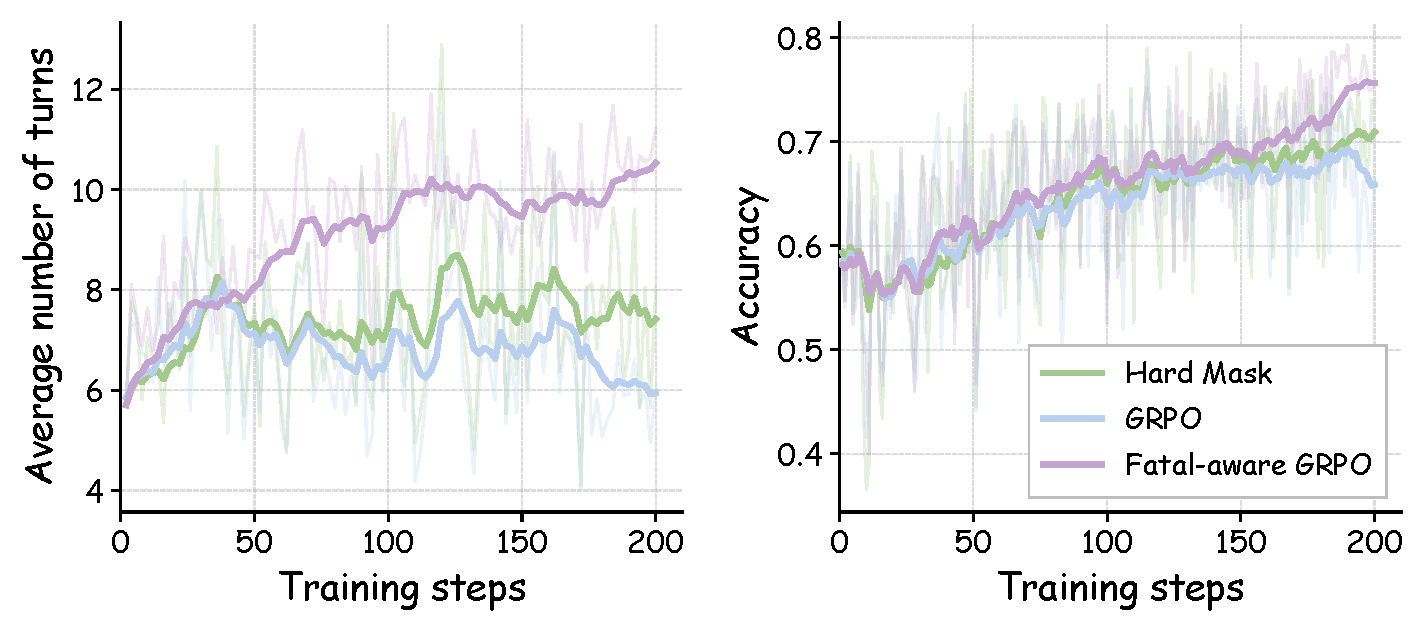
\includegraphics[width=0.84\linewidth]{figures/turn_acc_combined.pdf}
    \caption{Training dynamics over the RL phase. \textbf{Left:} average
    number of turns per rollout. \textbf{Right:} batch-level accuracy.
    Fatal-aware GRPO sustains a higher number of turns \emph{and} reaches a
    higher accuracy than vanilla GRPO~\citep{jin2025searchr1trainingllmsreason, guo2025deepseek} and the Hard-Mask~\citep{huang2026vision} baseline.}
    \label{fig:turn-acc-curves}
\end{figure}


\begin{figure}[!t]
  \centering
  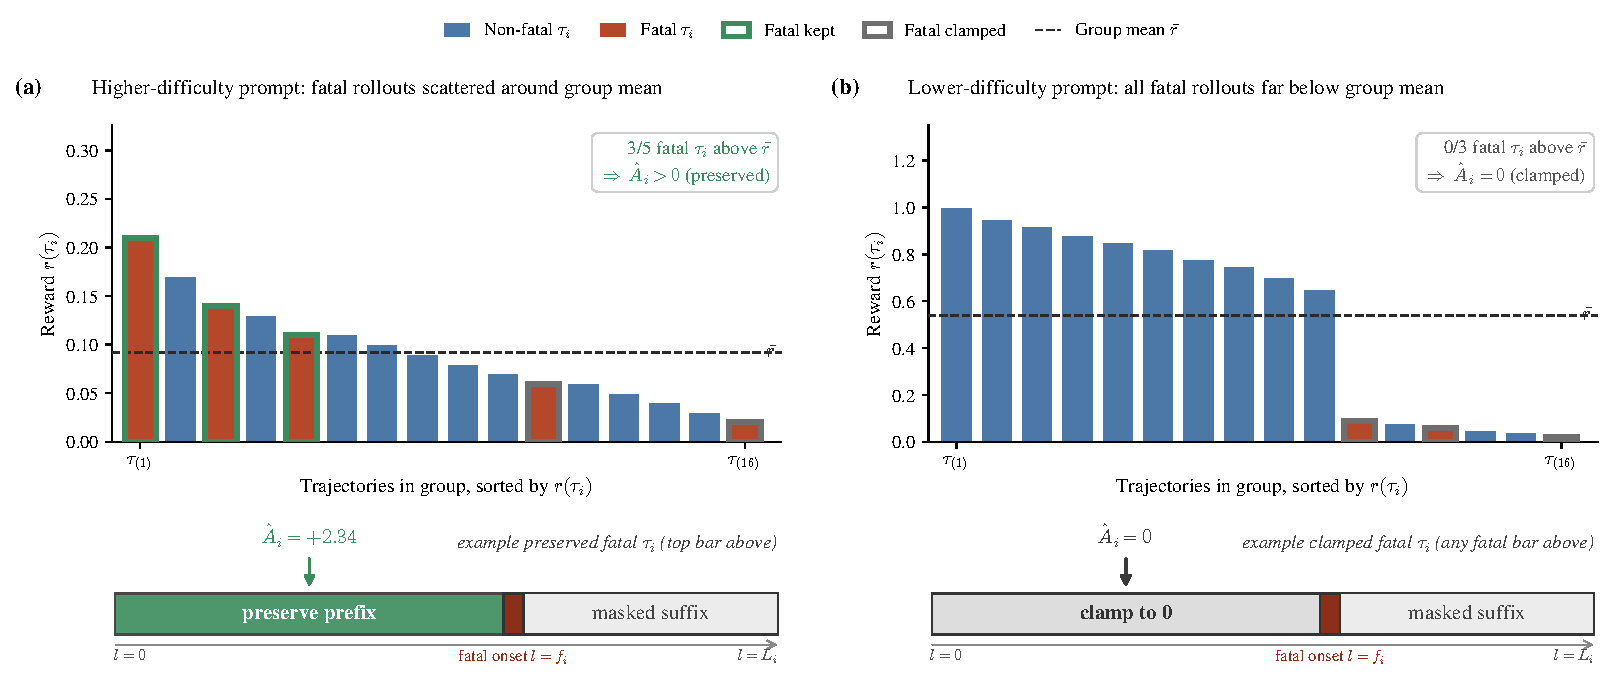
\includegraphics[width=0.92\linewidth]{figures/fatal_clamping_cases.pdf}
  \caption{\small%
    \textbf{Fatal-aware masking with one-sided clamping on two illustrative rollout groups.}
    Each panel shows a group of $G{=}16$ rollouts (non-fatal in blue, fatal in brick red) together with a cartoon of the resulting token-level update on one representative fatal trajectory $\tau_i$. Bar outlines mark fatal rollouts whose pre-clamp score $\widetilde{r}_i$ exceeds the group mean $\bar{r}$ (green, preserved) or falls below it (dark grey, clamped).
    \textbf{(a) Higher-difficulty prompt.} When $\bar{r}$ is low, several fatal prefixes already beat it: $\widetilde{r}_i > 0$ and $\hat{A}_i = \widetilde{r}_i$, so gradients flow only through the viable prefix (tokens up to the fatal onset $f_i$) while the post-failure suffix is hard-masked---the partial reasoning that reached the failure point is \emph{reinforced} even though the trajectory itself is unsolvable.
    \textbf{(b) Lower-difficulty prompt.} When most rollouts succeed, every fatal reward falls far below $\bar{r}$ and one-sided clamping sets $\hat{A}_i = \max(\widetilde{r}_i,0) = 0$, degenerating to pure hard-masking and avoiding any suppression of the possibly-valid prefix.%
  }
  \label{fig:fatal-clamping-cases}
\end{figure}

\paragraph{Empirical Visualization of the Two Cases.}
Figure~\ref{fig:fatal-clamping-cases} visualizes how $\hat{A}_i = \max(\widetilde{r}_i, 0)$ interacts with per-group difficulty on two representative rollout groups. In the higher-difficulty case, most fatal trajectories still emit a coherent prefix before hitting a tool error; a fraction of them beat the group mean and contribute a positive gradient to the prefix tokens only. In the lower-difficulty case, every fatal trajectory is dominated by the successful non-fatal rollouts, and clamping to zero prevents a noisy negative signal from pushing the policy \emph{away} from what may actually be a valid prefix.
Figure~\ref{fig:fatal-clamping-aggregate} shows that this split is not anecdotal: aggregated over $10{,}000$ groups, the vast majority of fatal trajectories sit on the negative side of the pre-clamp score and are safely zeroed out, while the small preserved tail is distributionally close to the right mode of the non-fatal reference. One-sided clamping thus recovers a principled credit signal from failed tool-call trajectories without amplifying their inherent noise.

